\documentclass{beamer}
\usepackage[utf8]{inputenc}
\usepackage{charter}
\usepackage{tikz}
\usepackage{graphicx}
\usepackage{amsmath}
\usepackage{amssymb}
\usepackage{blkarray}
\usepackage{subcaption}

%% Title slide formatting %%

\pgfdeclareimage[width=\paperwidth]{titlebackground}{title-slide-background.png}
\setbeamerfont{subtitle}{size=\tiny}
\setbeamertemplate{title page}{
    \begin{picture}(0,0)
        \put(-28.5,-163){%
            \pgfuseimage{titlebackground}
        }
        \put(0,-75){%
            \begin{minipage}[b][4.5cm][t]{0.5\textwidth}
                \color{white}
                \usebeamerfont{title}
                    {\inserttitle\\[0.9cm]}
                \usebeamerfont{subtitle}
                    {\insertauthor\par}
                    {\insertinstitute\\[0.3cm]}
                    {\insertdate}
            \end{minipage}
        }
    \end{picture}
}


%% General slide formatting %%

\definecolor{oxfordblue}{RGB}{4,30,66}

\pgfdeclareimage[width=1.2cm]{iitblogo}{iitb-logo.png}
%\pgfdeclareimage[width=1cm]{mathslogo}{mathematics-logo.png}

\setbeamertemplate{headline}
{%
    \begin{picture}(0,0)
        \put(314,-50){%
            \pgfuseimage{iitblogo}
        }
        \put(20,-55){%
            \rule{320pt}{0.4pt}
        }
    \end{picture}
}

\setbeamertemplate{frametitle}
{%
    \begin{picture}(0,0)
        \put(-8,-10){%
            \normalsize\color{oxfordblue}\insertframetitle
        }
        \put(-7,-20){%
            \tiny\color{oxfordblue}\insertframesubtitle
        }
    \end{picture}
}

\setbeamertemplate{footline}
{%
    \begin{picture}(0,0)
        \put(20,30){%
            \rule{320pt}{0.4pt}
        }
        % \put(20,14){%
        %     \pgfuseimage{mathslogo}
        % }
        % \put(100,14){%
        %     \color{oxfordblue}\insertshortdate
        % }
        \put(150,14){%
            \color{oxfordblue}\insertshorttitle
        }
        \put(337,14){%
            \color{oxfordblue}\insertpagenumber
        }
    \end{picture}%
}


%% Information (author, title, etc.) %%

\title[\textit{Contact-ing} the Schrödinger]{An Overview of the NEGF Formalism} % short title for footer
\author%
{%
    \sc{Debasish Panda}\\
    \sc{21d070021}
}
\institute%
{%
    \textit{Department of Electrical Engineering}\\
    \textit{Indian Institute of Technology, Bombay}
}
\date[2024]{UG RnD, May 2024}

%% Content of slides %%

\begin{document}

    \begin{frame}[plain]
        \titlepage
    \end{frame}


{
\usebackgroundtemplate{
\tikz[overlay,remember picture] 
\node[opacity=0.3, at=(current page.center)] {
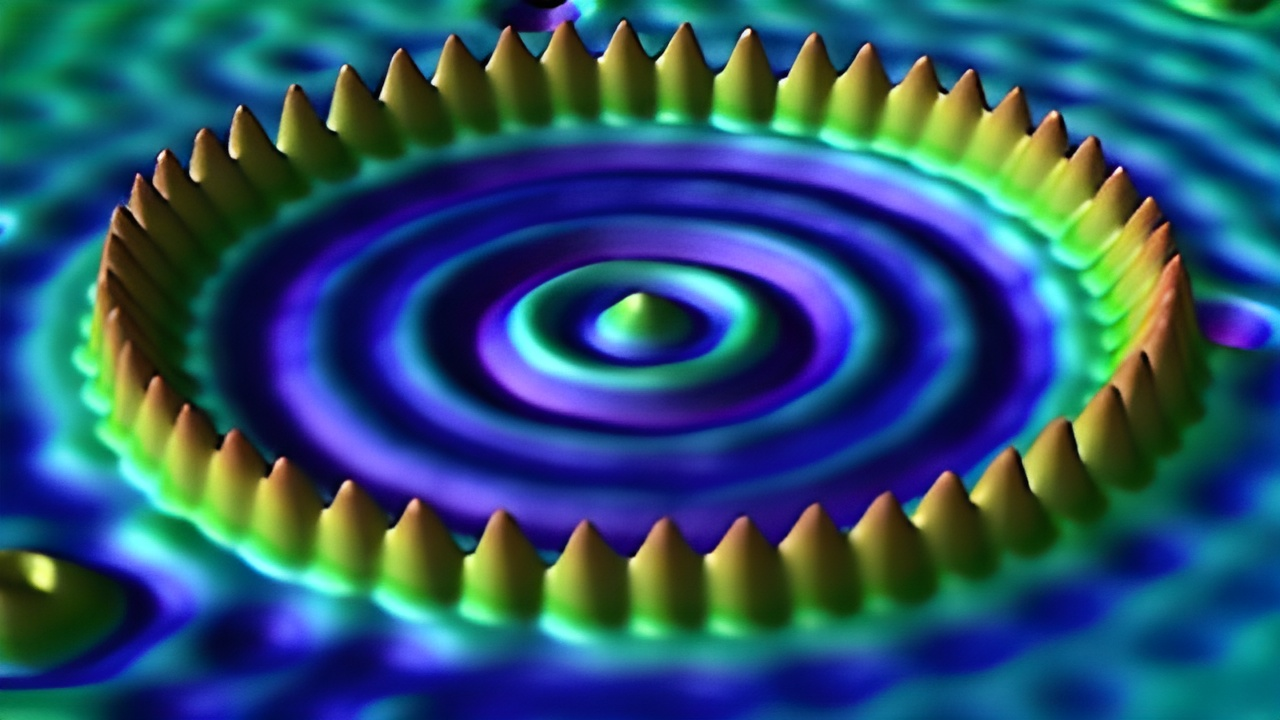
\includegraphics[height=\paperheight,width=\paperwidth]{cmp_2.jpeg} 
};}

    \begin{frame}

        \frametitle{NEGF formalism}
        \framesubtitle{Fundamental equations governing NEGF}
        \scriptsize

\vspace{30pt}

\begin{figure}[!htbp]
\centering
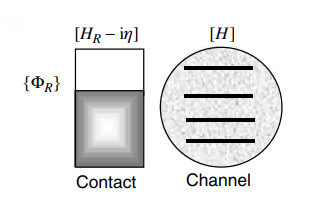
\includegraphics[scale=0.4]{ngef_1.png}
\caption{\scriptsize Channel contains no electrons and is disconnected from the contact where the electrons occupy the states described by $\{\Phi_{R}\}$}
\end{figure}
        
    \end{frame}
}


{
\usebackgroundtemplate{
\tikz[overlay,remember picture] 
\node[opacity=0.3, at=(current page.center)] {
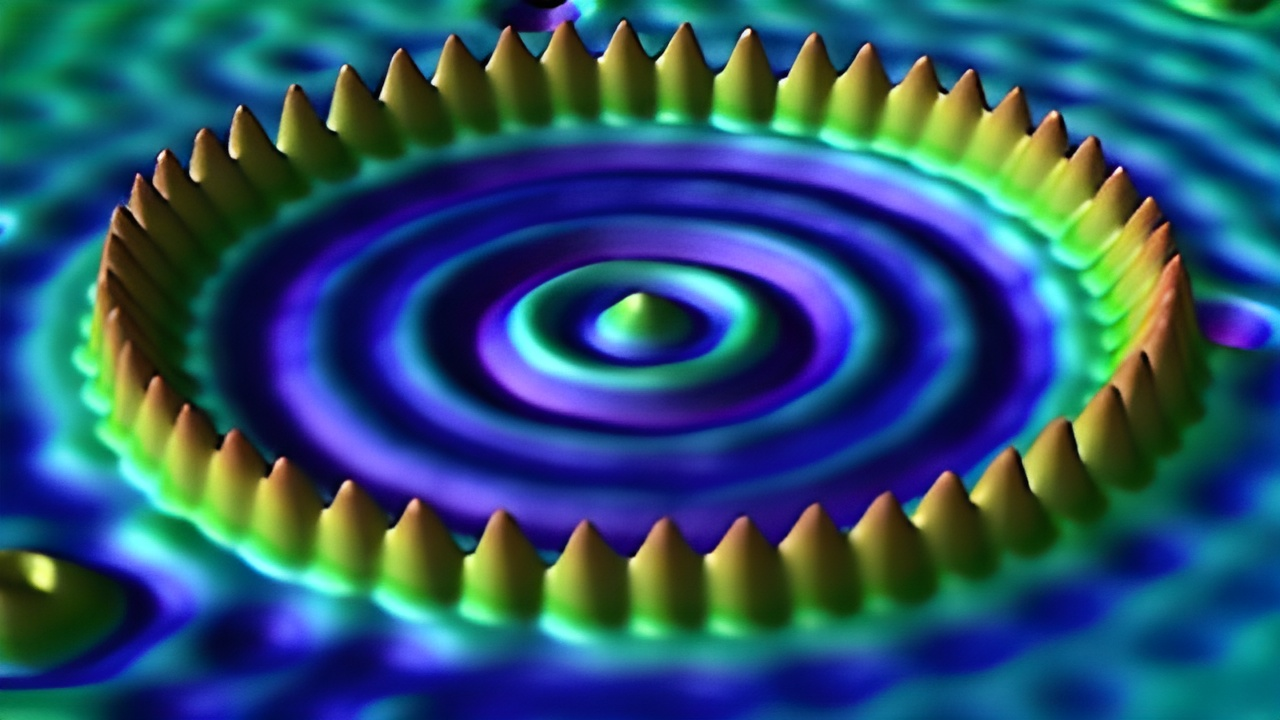
\includegraphics[height=\paperheight,width=\paperwidth]{cmp_2.jpeg} 
};}

    \begin{frame}

        \frametitle{NEGF formalism}
        \framesubtitle{Fundamental equations governing NEGF}
        \scriptsize

\vspace{12pt}
\begin{equation*}
\begin{blockarray}{ccc}
& \text{contact} & \text{device} \\
\begin{block}{c(cc)}
\text{contact} & EI_{R}-H_{R}+i\eta & -\tau^{\dagger} \\
\text{device} & -\tau & EI-H \\
\end{block}
\end{blockarray}
\begin{Bmatrix}
    \Phi_{R}+\chi \\
    \psi \\
\end{Bmatrix} = 
\begin{Bmatrix}
    S_{R} \\
    0 
\end{Bmatrix}
\end{equation*}

\begin{align*}
   G_{R} &= [EI_{R}-H_{R}+i\eta]^{-1} \\
   \{\chi\} &= G_{R}\ \tau^{\dagger}\{\psi\} \\
   \{\psi\} &= G \ \{S\} 
\end{align*}
where
\begin{align*}
    G &= [EI-H-\Sigma]^{-1} \\
    \Sigma &= \tau G_{R} \tau^{\dagger}, \quad S = \tau \Phi_{R}
\end{align*}
\vspace{-6pt}

    \end{frame}
}


{
\usebackgroundtemplate{
\tikz[overlay,remember picture] 
\node[opacity=0.3, at=(current page.center)] {
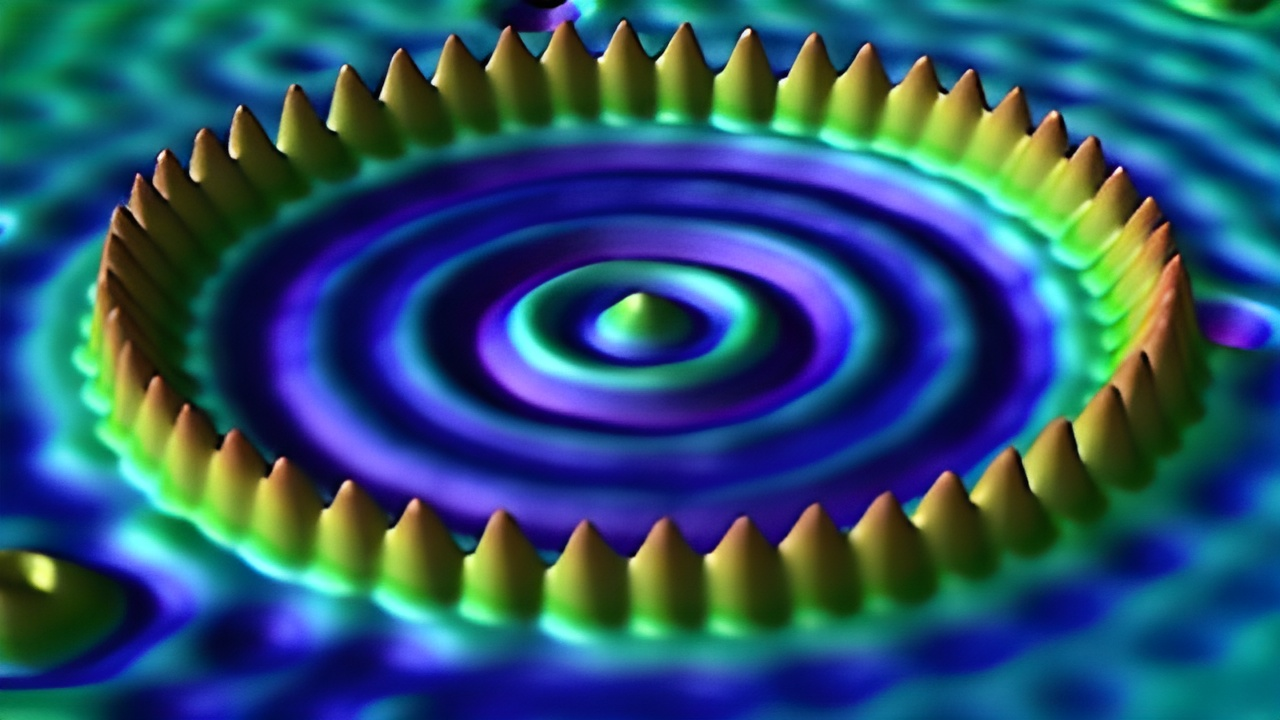
\includegraphics[height=\paperheight,width=\paperwidth]{cmp_2.jpeg} 
};}

    \begin{frame}
        \frametitle{NEGF formalism}
        \framesubtitle{Level broadening and LDOS}
        \scriptsize

\vspace{24pt}

The contact/reservoir has a near-continuous distribution of energy levels, whereas the channel has a discrete set of energy levels. When the channel is coupled to a contact, one would expect an intermediate state of such energy levels- something in between a continuous distribution and discrete levels. This also implies that the energy levels within the channel are no longer eigenvalues of the Hamiltonian, $[H]$, but act as independent variables. \par 

\begin{figure}[!htbp]
\centering
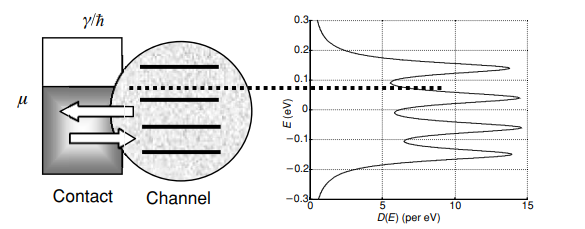
\includegraphics[scale=0.4]{level_broad.png}
\end{figure}

    \end{frame}
}


{
\usebackgroundtemplate{
\tikz[overlay,remember picture] 
\node[opacity=0.3, at=(current page.center)] {
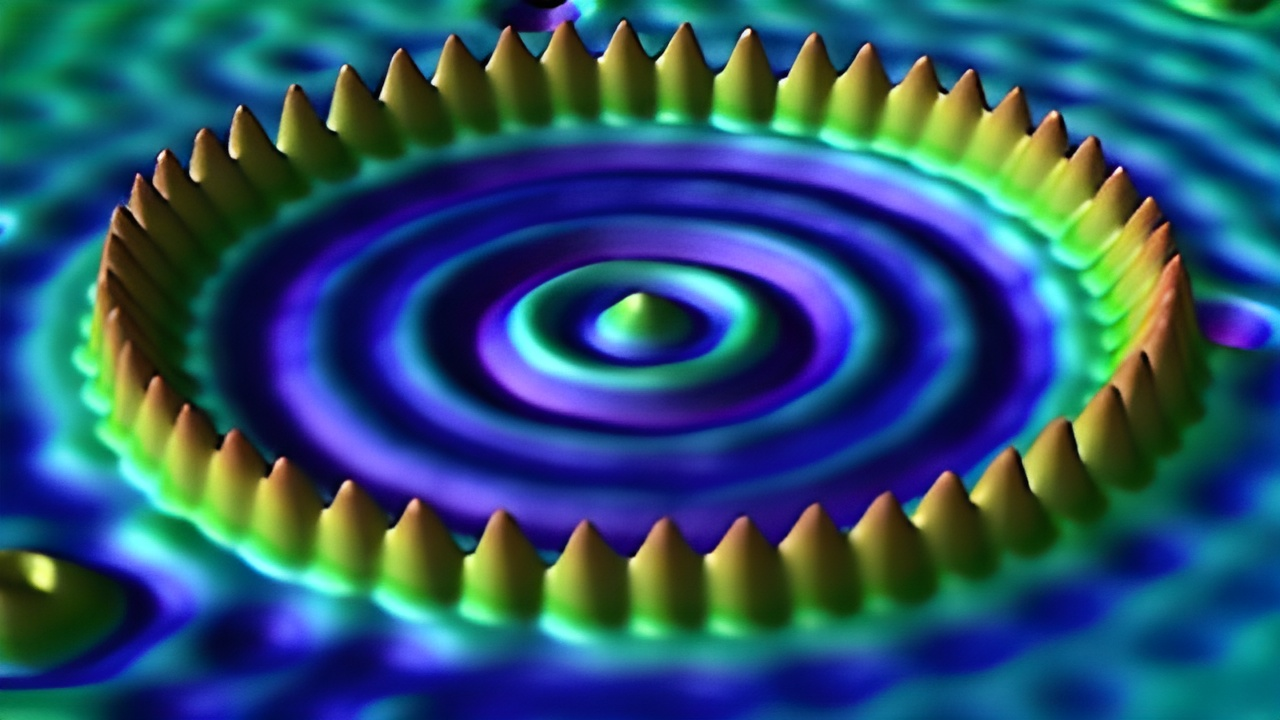
\includegraphics[height=\paperheight,width=\paperwidth]{cmp_2.jpeg} 
};}

    \begin{frame}

        \frametitle{NEGF formalism}
        \framesubtitle{Level broadening and LDOS}
        \scriptsize

LDOS:
\begin{equation*}
    D(\vec{r};E) = \sum_{\alpha}|\Phi_{\alpha}(\vec{r})|^{2} \  \delta(E-\epsilon_{\alpha}),
\end{equation*}
which is the diagonal element of the spectral matrix, $[A(E)]$:
\begin{equation*}
    A(\vec{r},\vec{r'};E) = 2\pi \sum_{\alpha}\phi_{\alpha}(\vec{r}) \ \delta(E-\epsilon_{\alpha}) \ \phi^{*}_{\alpha}(\vec{r'})
\end{equation*}
In matrix notation, $[A(E)] = 2\pi \delta(E[I]-[H])$, $D(E) = \frac{1}{2\pi}\text{Tr}[A(E)]$

        
    \end{frame}
}


{
\usebackgroundtemplate{
\tikz[overlay,remember picture] 
\node[opacity=0.3, at=(current page.center)] {
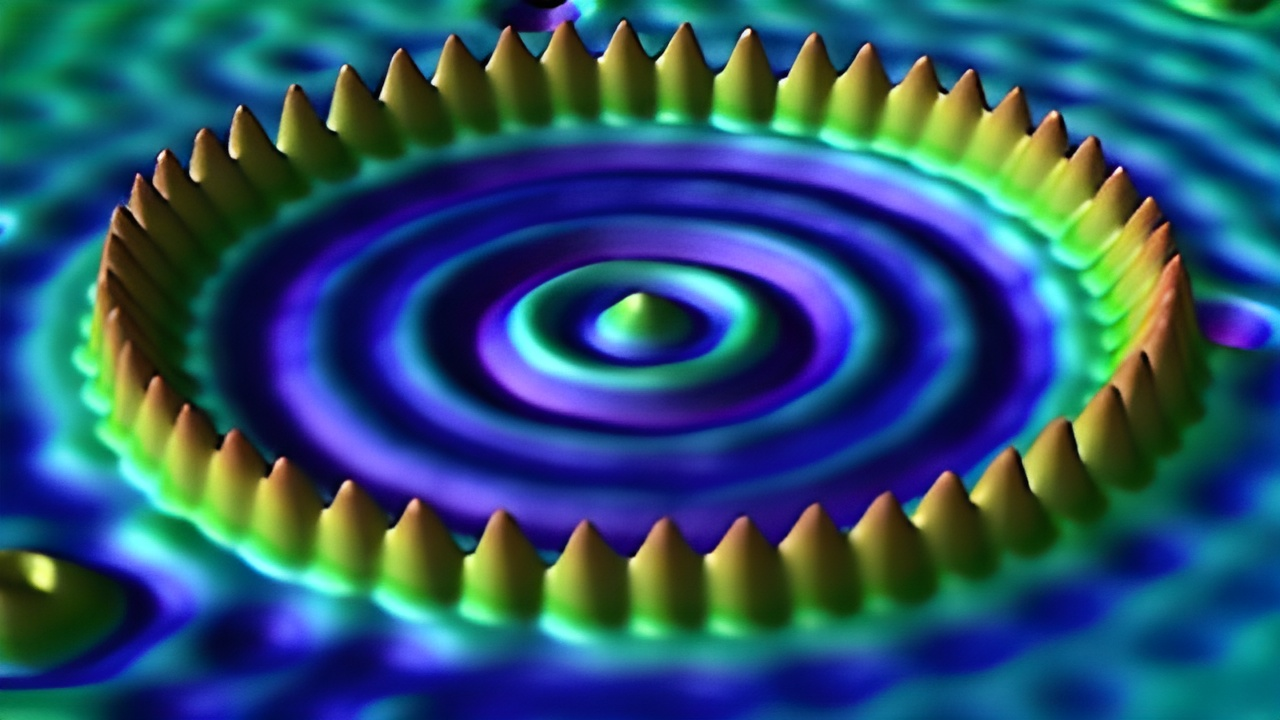
\includegraphics[height=\paperheight,width=\paperwidth]{cmp_2.jpeg} 
};}
    \begin{frame}

        \frametitle{NEGF formalism}
        \framesubtitle{Level broadening and LDOS}
        \scriptsize

\vspace{18pt}

\begin{equation*}
    2\pi \delta(E-\epsilon_{\alpha}) = \left[\frac{2\eta}{(E-\epsilon_{\alpha})^{2}+\eta^{2}} \right]_{\eta \rightarrow 0^+}
\end{equation*}
the spectral matrix can be expressed as:
\begin{equation*}
    [A(E)] = i[G(E)-G^{\dagger}(E)]
\end{equation*}
where 
\begin{align*}
    \text{Retarded Green's function}: G(E) &= [(E+i0^{+})I-H]^{-1} \\
    \text{Advanced Green's function}: G^{\dagger}(E) &= [(E-i0^{+})^{-1}I-H]^{-1}
\end{align*}
Note that the above expressions hold true for the reservoir/contact Green functions. The equivalent device/channel Green functions are given by:
\begin{align*}
    \text{Retarded Green's function}: G(E) &= [(E+i0^{+})I-H-\tau G_{R} \tau^{\dagger}]^{-1} \\
    \text{Advanced Green's function}: G^{\dagger}(E) &= [(E-i0^{+})^{-1}I-H-\tau G_{R} \tau^{\dagger}]^{-1}
\end{align*}

    \end{frame}
}


{
\usebackgroundtemplate{
\tikz[overlay,remember picture] 
\node[opacity=0.3, at=(current page.center)] {
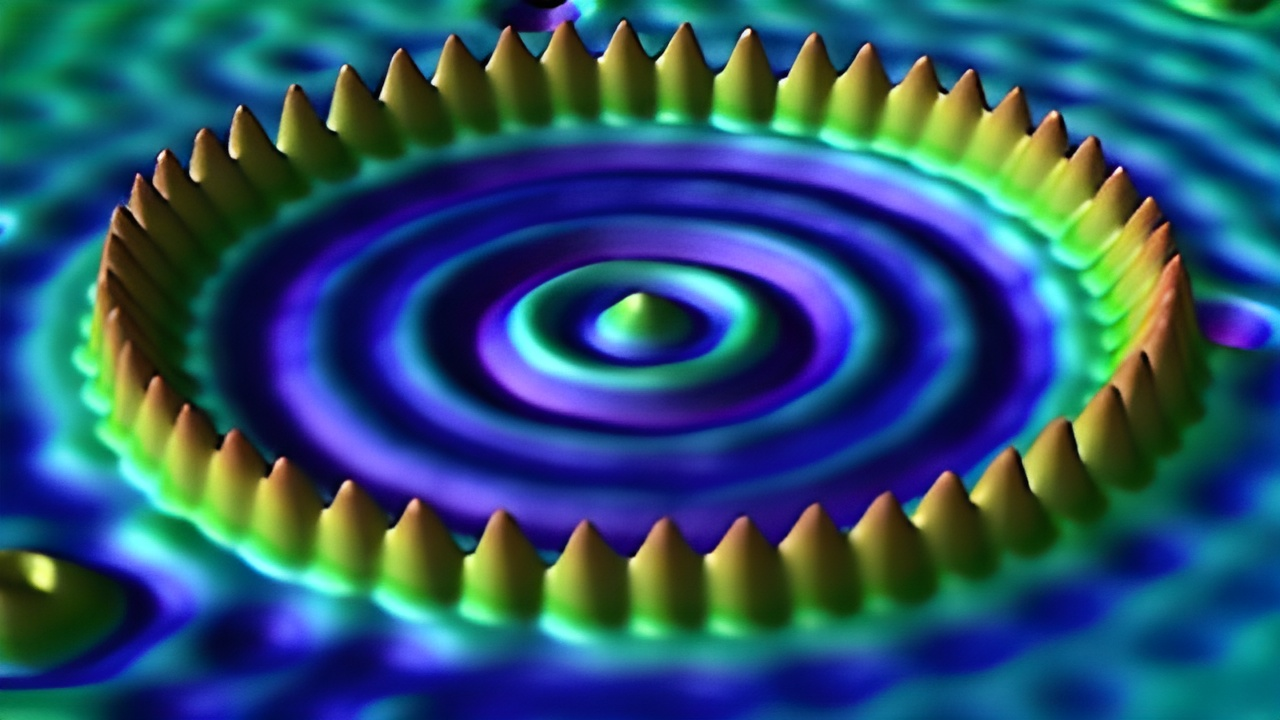
\includegraphics[height=\paperheight,width=\paperwidth]{cmp_2.jpeg} 
};}

    \begin{frame}
        
        \frametitle{NEGF formalism}
        \framesubtitle{Green's functions in time domain}
        \scriptsize

\vspace{12pt}

$[\tilde{G}^{R}(t)]$: Fourier transform of $[G^{R}(E)]$

\begin{equation*}
    [\tilde{G}^{R}(t)] = -\frac{i}{\hbar}\nu(t)e^{-i0^{+}t}
    \begin{bmatrix}
        e^{-i\epsilon_{1}t/\hbar} & 0 & 0 & \ldots \\
        0 & e^{-i\epsilon_{2}t/\hbar} & 0 & \ldots \\
        0 & 0 & e^{-i\epsilon_{3}t/\hbar} & \ldots \\
        \ldots & \ldots & \ldots & \ldots 
    \end{bmatrix}
\end{equation*}

Similarly, 
\begin{equation*}
    [\tilde{G}^{A}(t)] = \frac{i}{\hbar}\nu(-t)e^{i0^{+}t}
    \begin{bmatrix}
        e^{-i\epsilon_{1}t/\hbar} & 0 & 0 & \ldots \\
        0 & e^{-i\epsilon_{2}t/\hbar} & 0 & \ldots \\
        0 & 0 & e^{-i\epsilon_{3}t/\hbar} & \ldots \\
        \ldots & \ldots & \ldots & \ldots 
    \end{bmatrix}
\end{equation*}

    \end{frame}
}


{
\usebackgroundtemplate{
\tikz[overlay,remember picture] 
\node[opacity=0.3, at=(current page.center)] {
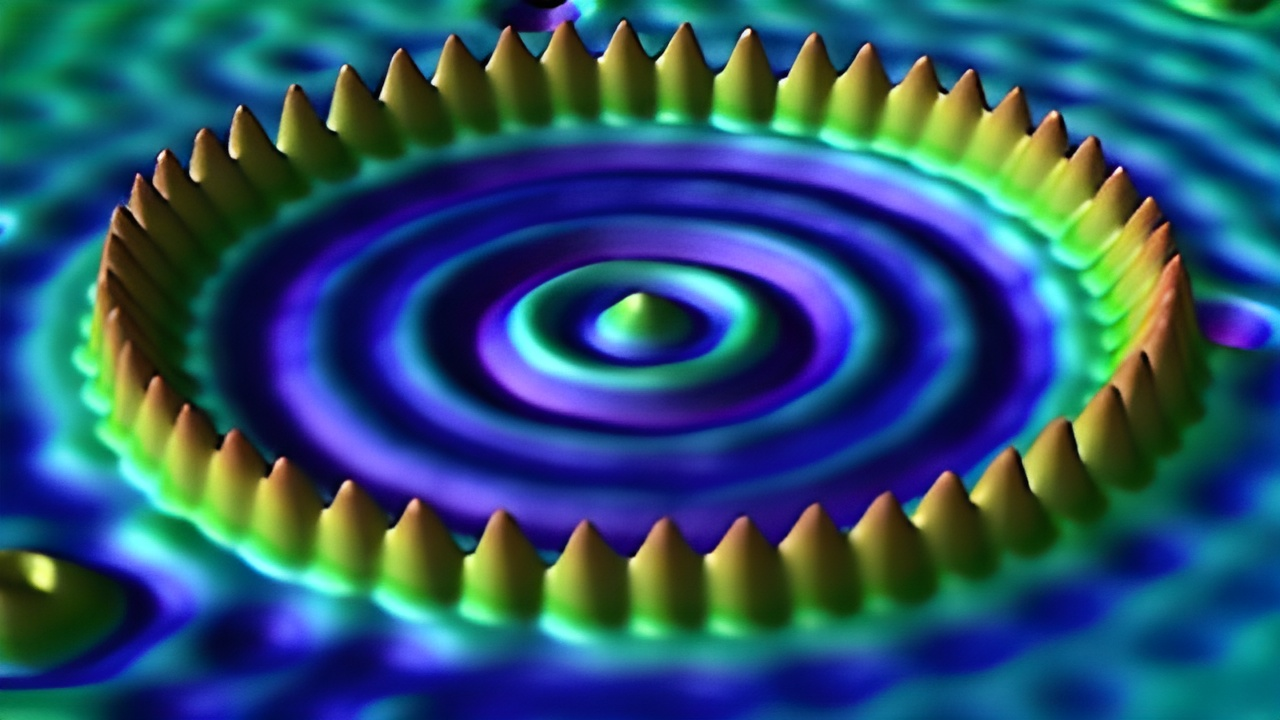
\includegraphics[height=\paperheight,width=\paperwidth]{cmp_2.jpeg} 
};}

    \begin{frame}

        \frametitle{NEGF formalism}
        \framesubtitle{Channel connected to two contacts}
        \scriptsize

\vspace{12pt}

\begin{figure}[!htbp]
\centering
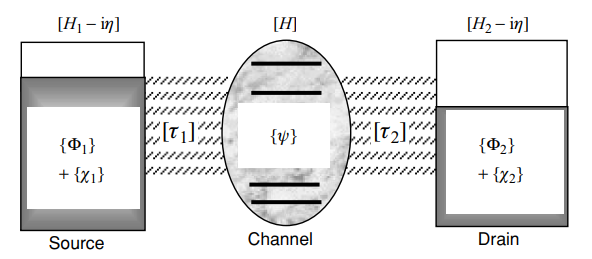
\includegraphics[scale=0.3]{two_contacts.png}
\end{figure}

\begin{equation*}
\begin{pmatrix}
    EI-H_{1}+i\eta & -\tau_{1}^{\dagger} & 0 \\
    -\tau_{1} & EI-H & -\tau_{2} \\
    0 & -\tau_{2}^{\dagger} & EI-H_{2}+i\eta
\end{pmatrix} 
\begin{Bmatrix}
    \Phi_{1}+\chi_{1} \\
    \psi \\
    \Phi_{2}+\chi_{2} 
\end{Bmatrix} =
\begin{Bmatrix}
    S_{1} \\ 
    0 \\
    S_{2}
\end{Bmatrix}
\end{equation*}

\vspace{6pt}

Channel Green's function, $G = [EI-H-\Sigma_{1}-\Sigma_{2}]^{-1}$ \\ \vspace{6pt}
Source term, $S = S_{1} + S_{2} = \tau_{1}\{\Phi_{1}\} + \tau_{2}\{\Phi_{2}\}$ \\ \vspace{6pt}
Spectral function, $A = A_{1}+A_{2} = G(\Gamma_{1}+\Gamma_{2})G^{\dagger}$

    \end{frame}
}


{
\usebackgroundtemplate{
\tikz[overlay,remember picture] 
\node[opacity=0.3, at=(current page.center)] {
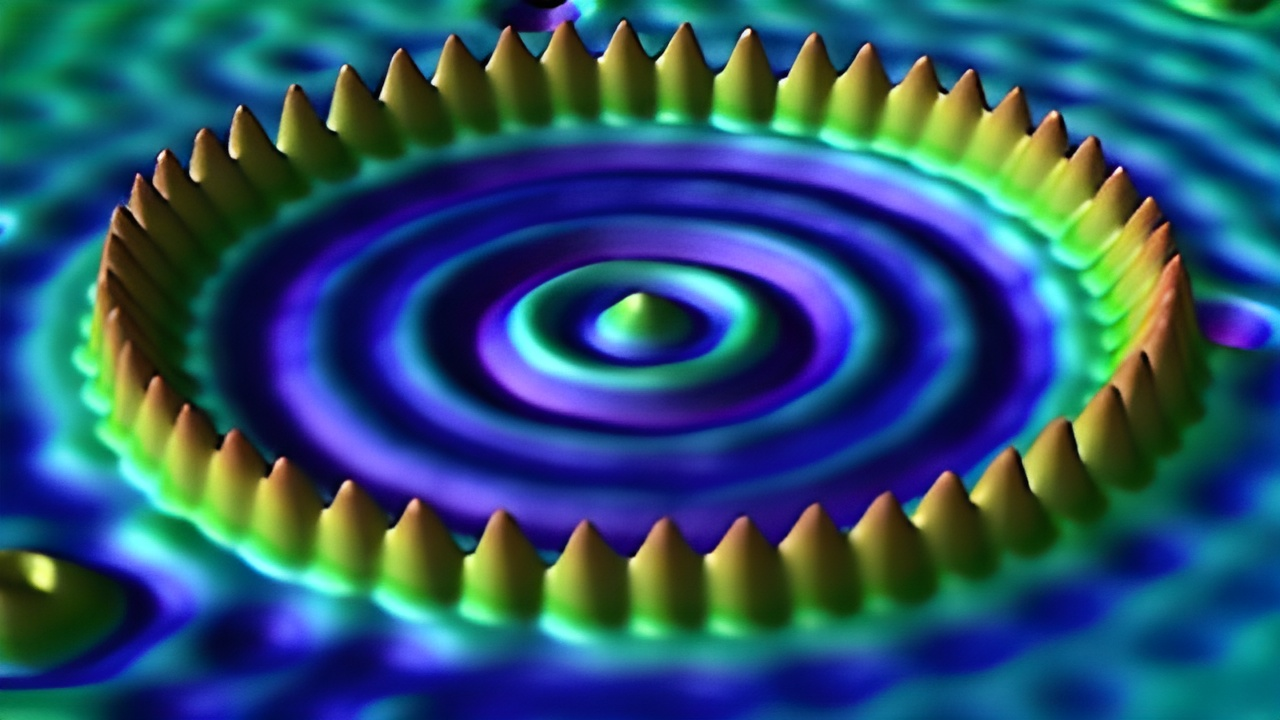
\includegraphics[height=\paperheight,width=\paperwidth]{cmp_2.jpeg} 
};}

    \begin{frame}
        \frametitle{NEGF formalism}
        \framesubtitle{Channel connected to two contacts}
        \scriptsize

\begin{align*}
    [\rho] &= \int_{-\infty}^{+\infty} \frac{dE}{2\pi}\ [G^{n}(E)] \\
    I_{i} &= -\frac{q}{h} \int_{-\infty}^{+\infty}dE\ \{\underbrace{\text{Tr}[\Gamma_{i}A]f_{i}}_\text{Inflow}-\underbrace{\text{Tr}[\Gamma_{i}G^{n}]}_\text{Outflow}\} \\
    \overline{T}(E) &= \text{Tr}[\Gamma_{2}G\Gamma_{1}G^{\dagger}]
\end{align*} 
where $[G^{n}] = [A_{1}]f_{1} + [A_{2}]f_{2} = G\Sigma_{in}G^{\dagger} = G\{[\Gamma_{1}]f_{1}+[\Gamma_{2}]f_{2}\}G^{\dagger}$

    \end{frame}
}


{
\usebackgroundtemplate{
\tikz[overlay,remember picture] 
\node[opacity=0.3, at=(current page.center)] {
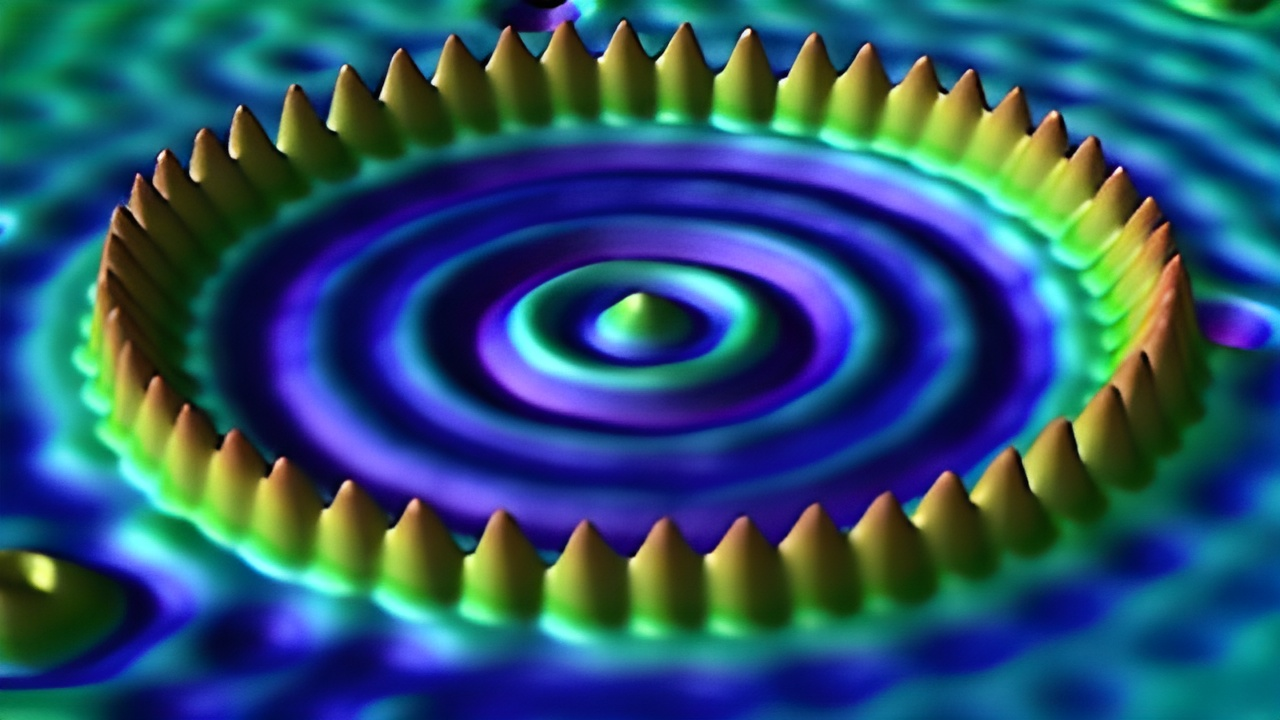
\includegraphics[height=\paperheight,width=\paperwidth]{cmp_2.jpeg} 
};}

    \begin{frame}
        \frametitle{NEGF formalism}
        \framesubtitle{1-D examples}
        \scriptsize

\begin{figure}
  \begin{subfigure}{0.3\textwidth}
    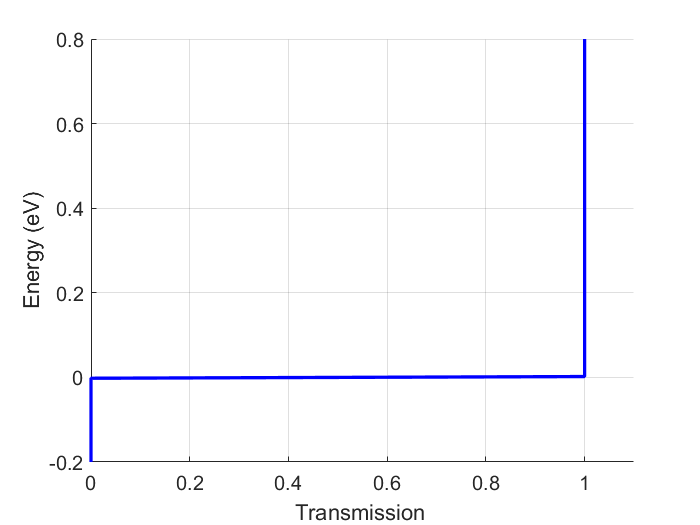
\includegraphics[width=\linewidth]{T_ballistic.png}
    \caption{\scriptsize Ballistic device}
  \end{subfigure}
  \begin{subfigure}{0.3\textwidth}
    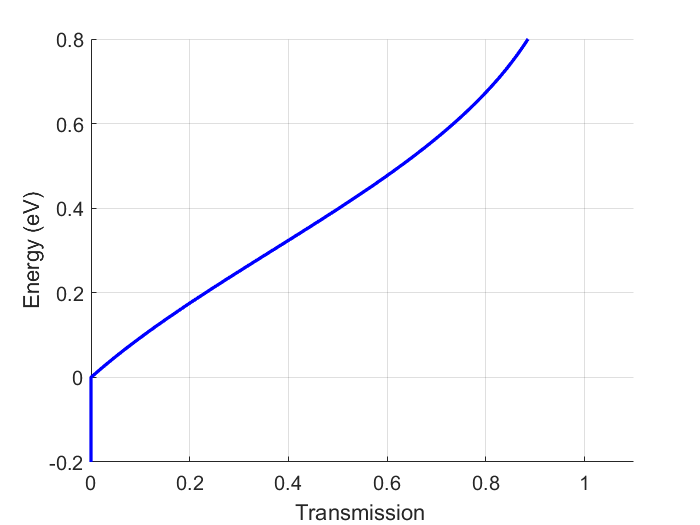
\includegraphics[width=\linewidth]{T_tunnel.png}
    \caption{\scriptsize Tunneling device}
  \end{subfigure}
  \begin{subfigure}{0.3\textwidth}
     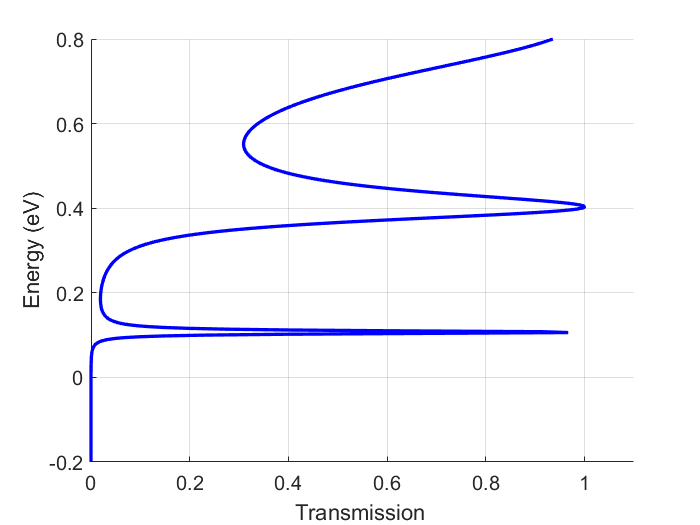
\includegraphics[width=\linewidth]{T_rtd.png}
     \caption{\scriptsize RTD}
  \end{subfigure}
  \caption{\scriptsize Transmission function for different devices}
\end{figure}
          
    \end{frame} 
} 


{
\usebackgroundtemplate{
\tikz[overlay,remember picture] 
\node[opacity=0.3, at=(current page.center)] {
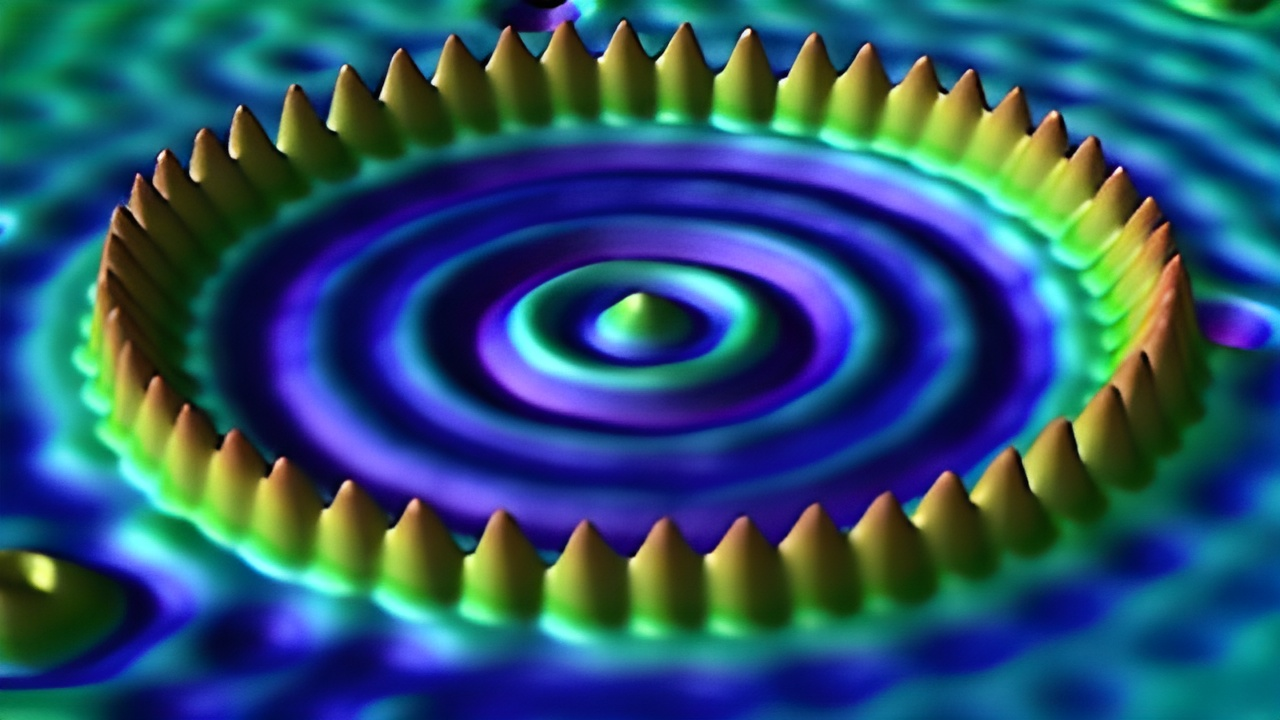
\includegraphics[height=\paperheight,width=\paperwidth]{cmp_2.jpeg} 
};}

    \begin{frame}
        \frametitle{NEGF formalism}
        \framesubtitle{1-D examples}
        \scriptsize

\begin{figure}
  \begin{subfigure}{0.3\textwidth}
    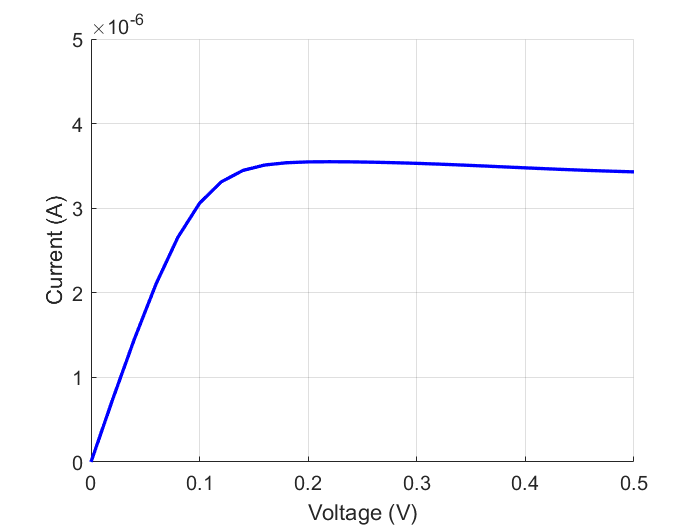
\includegraphics[width=\linewidth]{IV_ballistic.png}
    \caption{\scriptsize Ballistic device}
  \end{subfigure}
  \begin{subfigure}{0.3\textwidth}
    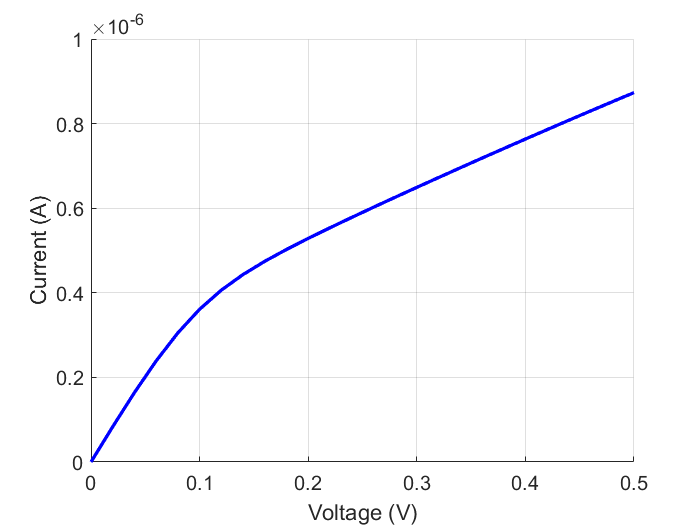
\includegraphics[width=\linewidth]{IV_tunnel.png}
    \caption{\scriptsize Tunneling device}
  \end{subfigure}
  \begin{subfigure}{0.3\textwidth}
     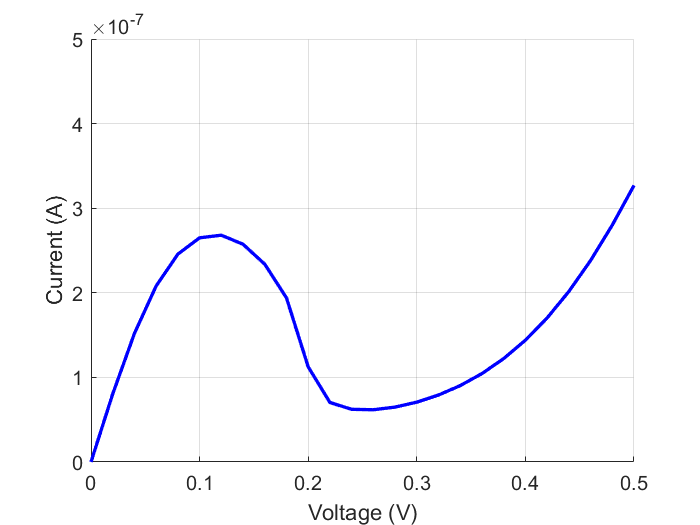
\includegraphics[width=\linewidth]{IV_rtd.png}
     \caption{\scriptsize RTD}
  \end{subfigure}
  \caption{\scriptsize I-V characteristics for different devices}
\end{figure}
          
    \end{frame} 
} 


{
\usebackgroundtemplate{
\tikz[overlay,remember picture] 
\node[opacity=0.3, at=(current page.center)] {
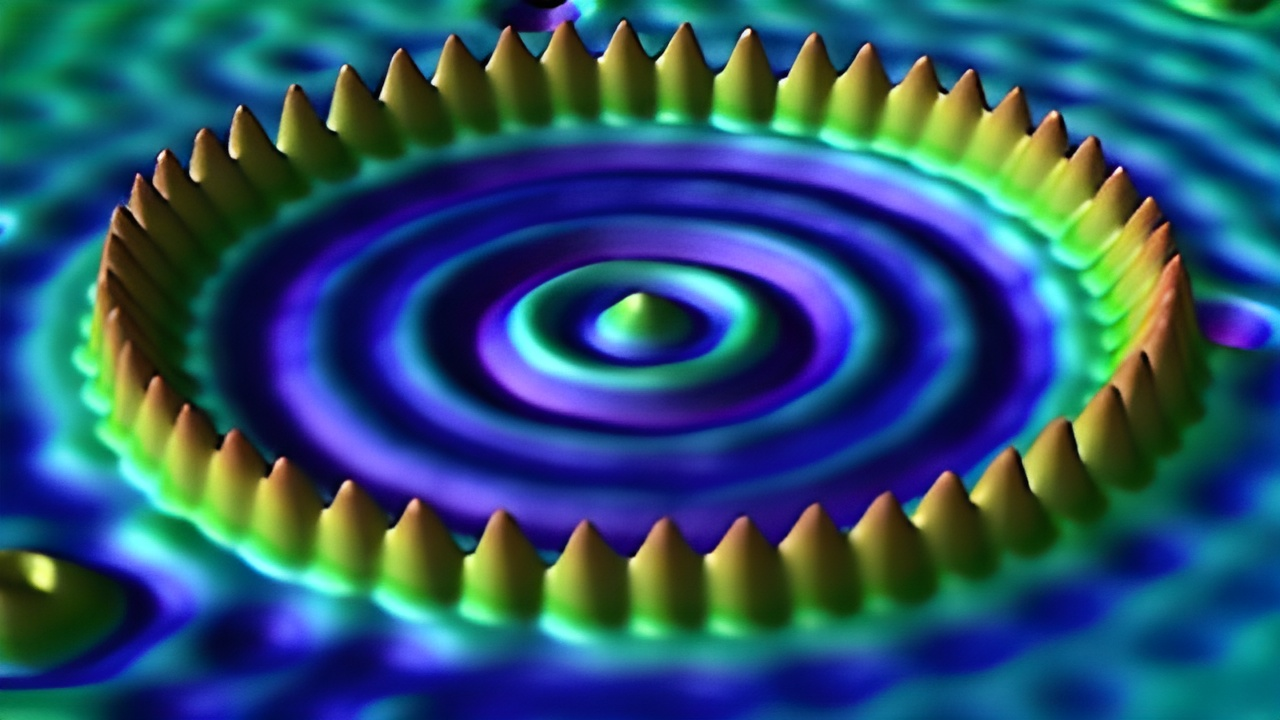
\includegraphics[height=\paperheight,width=\paperwidth]{cmp_2.jpeg} 
};}

    \begin{frame}
        \frametitle{NEGF formalism}
        \framesubtitle{2-D conductors}
        \scriptsize

\vspace{12pt}

\begin{figure}[!htbp]
   \begin{subfigure}{0.15\textwidth}
   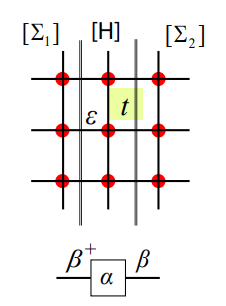
\includegraphics[width=\linewidth]{2d_init_basis.png}
   \end{subfigure}
   \hspace{1cm}
   \begin{subfigure}{0.15\textwidth}
   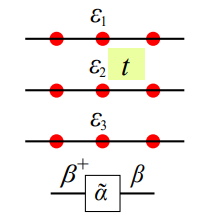
\includegraphics[width=\linewidth]{2d_change_basis.png}
   \end{subfigure}
\end{figure}
         
where 
\begin{equation*}
    \alpha = \begin{bmatrix}
             \epsilon & t & 0 \\
             t & \epsilon & t \\
             0 & t & \epsilon 
             \end{bmatrix}, \
    \beta = \begin{bmatrix}
            t & 0 & 0 \\
            0 & t & 0 \\
            0 & 0 & t
            \end{bmatrix}
\end{equation*}
A basis transformation can be done such that $\alpha$ is diagonalized: 
\begin{equation*}
    \tilde{\alpha} = V^{\dagger}\alpha V, \quad \tilde{\beta} = \beta
\end{equation*}
In the transformed basis, the 2D conductors can be visualized as a set of independent 1D conductors, with diagonal elements $\epsilon_{n} = \epsilon-2t\ cos(k_{n}a)$, where $k_{n}a = \frac{n\pi}{N+1}$.

    \end{frame} 
}


{
\usebackgroundtemplate{
\tikz[overlay,remember picture] 
\node[opacity=0.3, at=(current page.center)] {
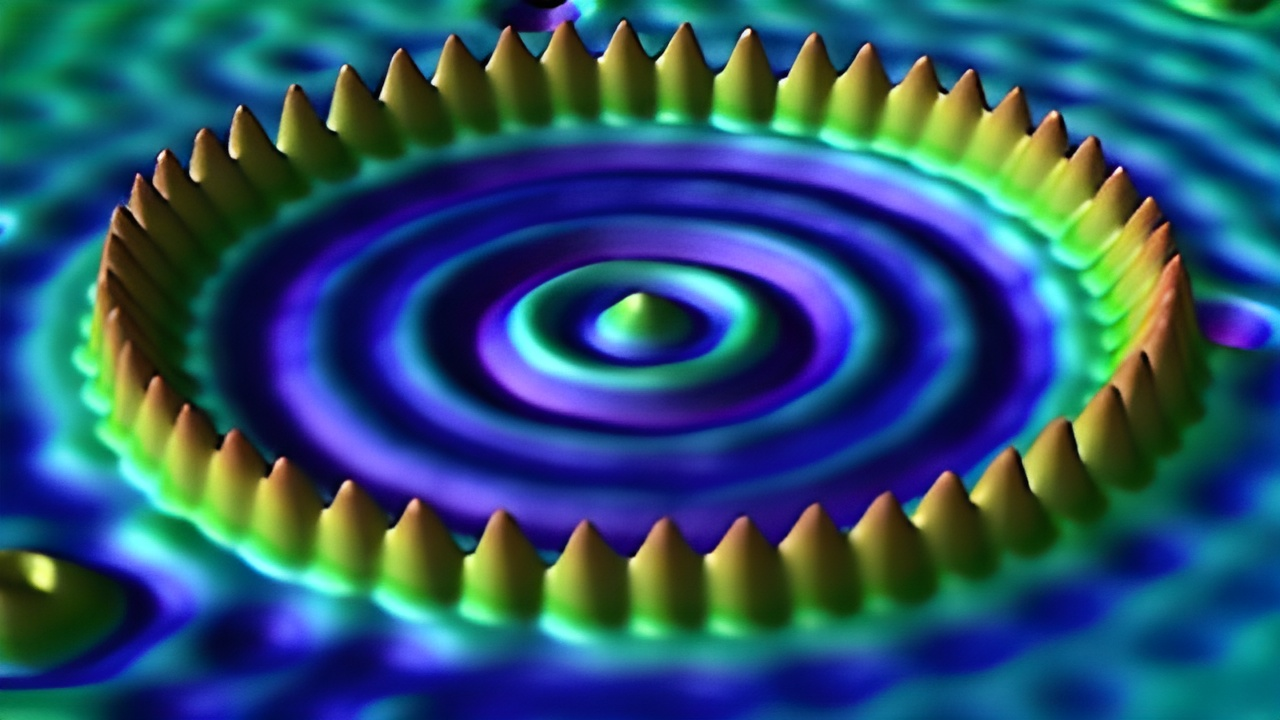
\includegraphics[height=\paperheight,width=\paperwidth]{cmp_2.jpeg} 
};}

    \begin{frame}
        \frametitle{NEGF formalism}
        \framesubtitle{2-D conductors}
        \scriptsize

Previously shown transformations convert the lattice basis to an abstract mode basis.
\begin{align*}
   \underbrace{\tilde{X}}_\text{Mode basis} &= V^{\dagger} \underbrace{X}_\text{Lattice basis} V \\ 
   \underbrace{X}_\text{Lattice basis} &= V \underbrace{\tilde{\text{X}}}_\text{Mode basis} V^{\dagger}
\end{align*}
\begin{equation*}
    \tilde{\Sigma}_{1} = \begin{bmatrix}
                         te^{ik_{1}a} & 0 & 0 & \ldots \\
                         0 & te^{ik_{2}a} & 0 & \ldots \\
                         0 & 0 & te^{ik_{3}a} & \ldots \\
                         \vdots & \vdots & \vdots & \ddots
                         \end{bmatrix}
\end{equation*}

    \end{frame} 
}


{
\usebackgroundtemplate{
\tikz[overlay,remember picture] 
\node[opacity=0.3, at=(current page.center)] {
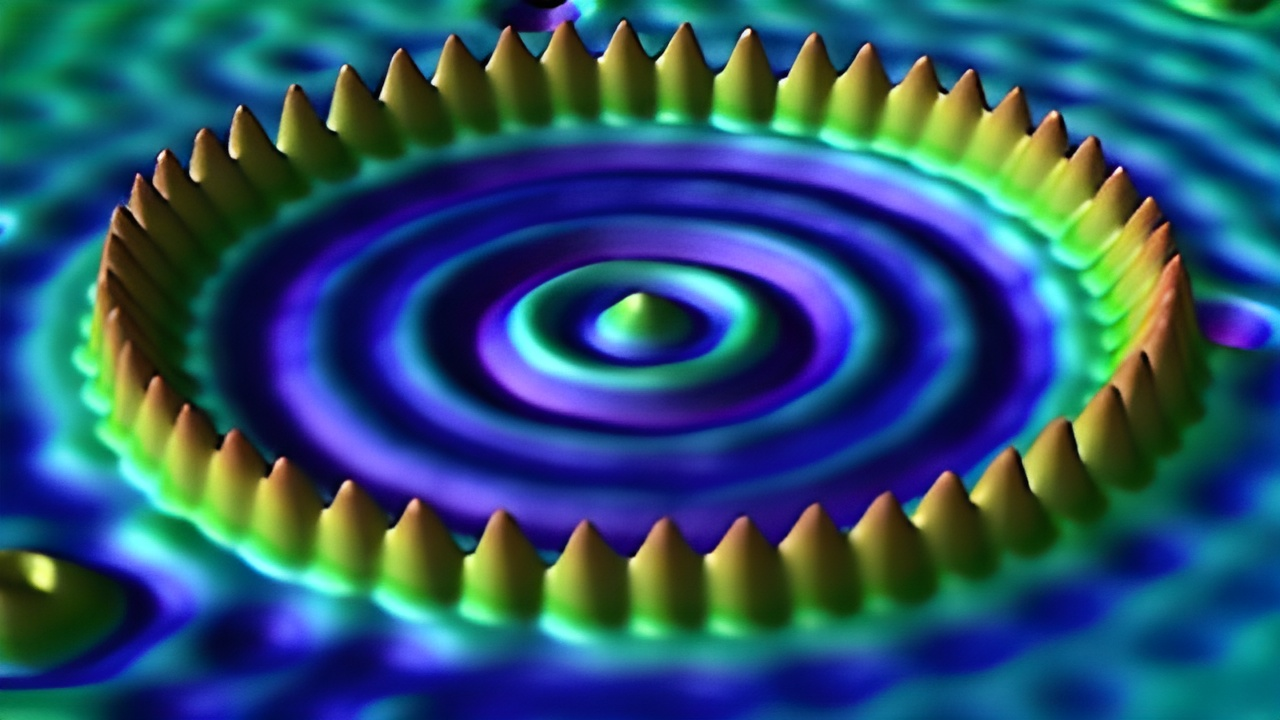
\includegraphics[height=\paperheight,width=\paperwidth]{cmp_2.jpeg} 
};}

    \begin{frame}
        \frametitle{NEGF formalism}
        \framesubtitle{Graphene}
        \scriptsize

\vspace{12pt}

\begin{figure}[!htbp]
\centering
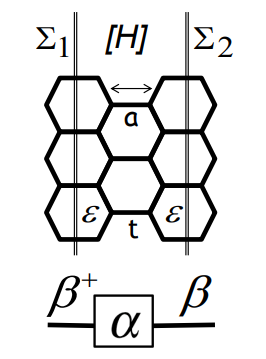
\includegraphics[scale=0.2]{graphene.png}
\end{figure}

Recursive relation:
\begin{equation*}
    g^{-1}_{2} = (E+i0^{+})I-\alpha-\beta^{\dagger}g_{2}\beta
\end{equation*}

    \end{frame} 
}


{
\usebackgroundtemplate{
\tikz[overlay,remember picture] 
\node[opacity=0.3, at=(current page.center)] {
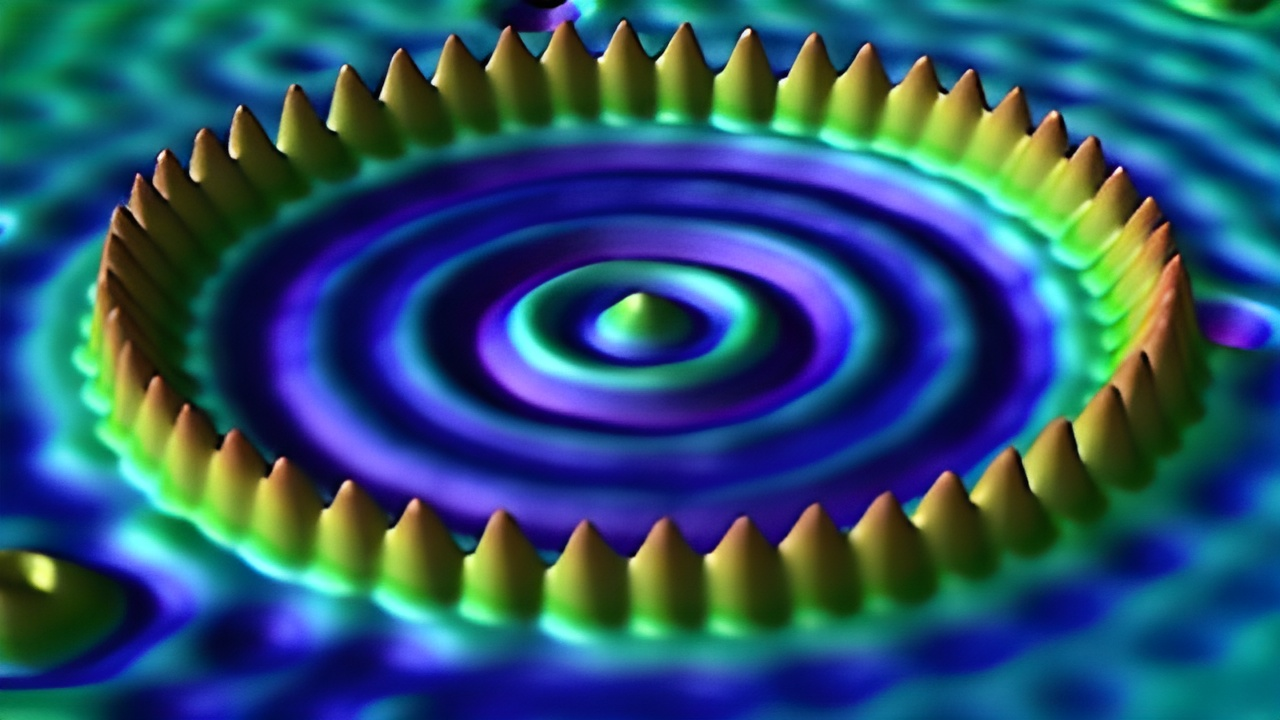
\includegraphics[height=\paperheight,width=\paperwidth]{cmp_2.jpeg} 
};}

    \begin{frame}
        \frametitle{NEGF formalism}
        \framesubtitle{Graphene}
        \scriptsize

\vspace{12pt}

\begin{figure}[!htbp]
   \begin{subfigure}{0.2\textwidth}
   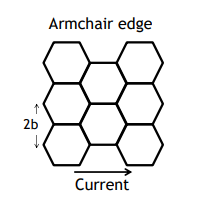
\includegraphics[width=\linewidth]{armchair.png}
   \end{subfigure}
   \hspace{0.5cm}
   \begin{subfigure}{0.2\textwidth}
   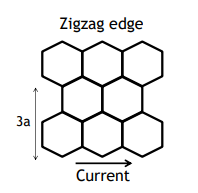
\includegraphics[width=\linewidth]{zigzag.png}
   \end{subfigure}
\end{figure}

\begin{figure}[!htbp]
   \begin{subfigure}{0.35\textwidth}
   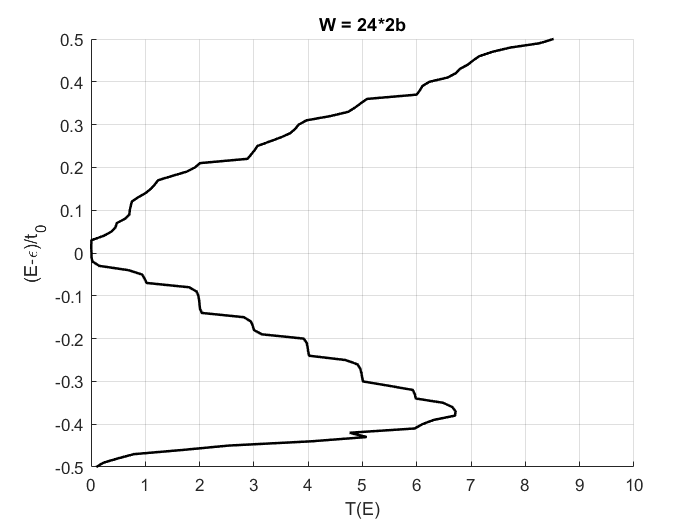
\includegraphics[width=\linewidth]{T_armchair.png}
   \end{subfigure}
   \hspace{0.5cm}
   \begin{subfigure}{0.35\textwidth}
   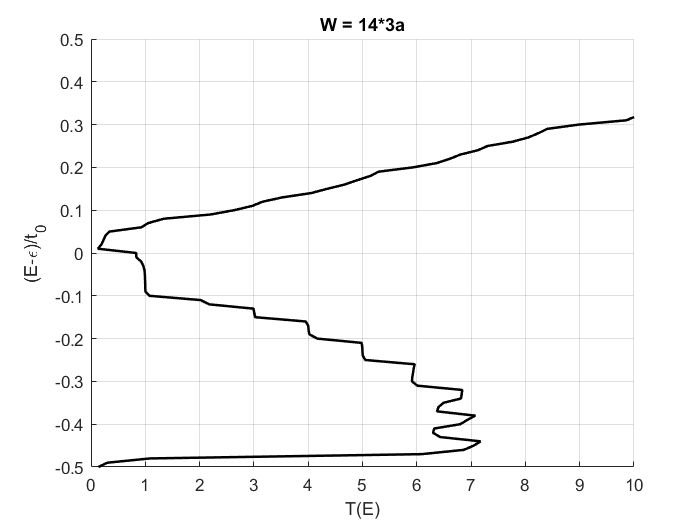
\includegraphics[width=\linewidth]{T_zigzag.png}
   \end{subfigure}
\end{figure}

    \end{frame} 
}


\end{document}